\documentclass{article}

\usepackage{amsmath}
\usepackage{amsthm}
\usepackage{amsfonts}
\usepackage{thmtools}
\usepackage{stmaryrd}
\usepackage{natbib}
\usepackage{url}
\usepackage{array}
\usepackage{arydshln}
\usepackage{ifthen}
\usepackage{ifpdf}


\usepackage{tikz}
\usepackage{multirow}

\declaretheorem[numbered=yes,name=Lemma]{lemma}
\declaretheorem[numbered=yes,name=Definition]{definition}
\declaretheorem[numbered=yes,name=Specification]{specification}

\newcommand{\forcenewline}{$\phantom{v}$\\}

\newcommand{\update}[2]{[#1 \mapsto #2]}
\newcommand{\sem}[1]{\left\llbracket #1 \right\rrbracket}

%Math notation
\newcommand{\restrictfun}[1]{|_{#1}}
\newcommand{\parfun}{\rightharpoonup}
\newcommand{\monnefun}{\stackrel{\textit{\tiny{mon, ne}}}{\longrightarrow}}
\newcommand{\monfun}{\stackrel{\textit{\tiny{mon}}}{\longrightarrow}}
\newcommand{\defeq}{\stackrel{\textit{\tiny{def}}}{=}}
\newcommand{\nequal}[1][n]{\stackrel{\tiny{#1}}{=}}
\newcommand{\nsubeq}[1][n]{\stackrel{\tiny{#1}}{\subseteq}}
\newcommand{\nsupeq}[1][n]{\stackrel{\tiny{#1}}{\supseteq}}
\newcommand{\union}{\mathbin{\cup}}
\DeclareMathOperator{\dom}{dom}

\newcommand{\undefined}{\mathit{undefined}}

\newcommand{\false}{\mathit{false}}
\newcommand{\true}{\mathit{true}}

%Comments
\newcommand\lau[1]{{\color{purple} \sf \footnotesize {LS: #1}}}
\newcommand\dominique[1]{{\color{purple} \sf \footnotesize {DD: #1}}}

%Variables
\newcommand{\var}[1]{\mathit{#1}}
\newcommand{\hs}{\var{hs}}
\newcommand{\hv}{\var{hv}}
\newcommand{\rv}{\var{rv}}
\newcommand{\lv}{\var{lv}}
\newcommand{\pc}{\mathit{pc}}
\newcommand{\pcreg}{\mathrm{pc}}
\newcommand{\addr}{\var{a}}
\newcommand{\offset}{\var{offset}}
\newcommand{\word}{\var{w}}
\newcommand{\start}{\var{base}}
\newcommand{\addrend}{\var{end}}
\newcommand{\mem}{\var{mem}}
\newcommand{\reg}{\var{reg}}
\newcommand{\heapseg}{\var{hs}}
\newcommand{\heap}{\var{heap}}
\newcommand{\mode}{\var{mode}}
\newcommand{\perm}{\var{perm}}

\newcommand{\stdcap}[1][\perm]{\left(#1,\start,\addrend,\addr \right)}

%Memory projections
\newcommand{\plainproj}[1]{\mathrm{#1}}
\newcommand{\memheap}[1][\Phi]{#1.\plainproj{heap}}
\newcommand{\memreg}[1][\Phi]{#1.\plainproj{reg}}

\newcommand{\updateHeap}[3][\Phi]{#1\update{\plainproj{heap}.#2}{#3}}
\newcommand{\updateReg}[3][\Phi]{#1\update{\plainproj{reg}.#2}{#3}}

%Configuration end states
\newcommand{\failed}{\textsl{failed}}
\newcommand{\halted}{\textsl{halted}}

%Functions
\newcommand{\plainfun}[1]{\mathit{#1}}
\newcommand{\decode}{\plainfun{decode}}
\newcommand{\encode}{\plainfun{encode}}
\newcommand{\encodePerm}{\plainfun{encodePerm}}
\newcommand{\updatePcPerm}[1]{\plainfun{updatePcPerm}(#1)}

\newcommand{\executeAllowed}[1]{\plainfun{executeAllowed}(#1)}
\newcommand{\nonZero}[1]{\plainfun{nonZero}(#1)}
\newcommand{\readAllowed}[1]{\plainfun{readAllowed}(#1)}
\newcommand{\writeAllowed}[1]{\plainfun{writeAllowed}(#1)}
\newcommand{\withinBounds}[1]{\plainfun{withinBounds}(#1)}
\newcommand{\stdUpdatePc}[1]{\plainfun{updatePc(#1)}}

\newcommand{\readCond}[1]{\plainfun{readCondition}(#1)}
\newcommand{\writeCond}[1]{\plainfun{readWriteCondition}(#1)}
\newcommand{\execCond}[1]{\plainfun{executeCondition}(#1)}
\newcommand{\entryCond}[1]{\plainfun{entryCondition}(#1)}


%World operations
\newcommand{\future}{\mathbin{\sqsupseteq}}
\newcommand{\heapSat}[3][\heap]{#1 :_{#2} #3}

%Assembly labels
\newcommand{\codelabel}[1]{\mathit{#1}}
\newcommand{\init}{\codelabel{init}}
\newcommand{\malloc}{\codelabel{malloc}}
\newcommand{\counter}{\codelabel{counter}}
\newcommand{\iocap}{\codelabel{iocap}}

%Type(s)
\newcommand{\type}[1]{\mathrm{#1}}
\newcommand{\asmType}{\plaindom{AsmType}}


%Domains
\newcommand{\plaindom}[1]{\mathrm{#1}}
\newcommand{\Caps}{\plaindom{Cap}}
\newcommand{\Words}{\plaindom{Word}}
\newcommand{\Addrs}{\plaindom{Addr}}
\newcommand{\Mems}{\plaindom{Mem}}
\newcommand{\RegName}{\plaindom{RegisterName}}
\newcommand{\Regs}{\plaindom{Reg}}
\newcommand{\Heaps}{\plaindom{Heap}}
\newcommand{\HeapSegments}{\plaindom{HeapSegment}}
\newcommand{\Confs}{\plaindom{Conf}}
\newcommand{\Instrs}{\plaindom{Instructions}}
\newcommand{\nats}{\mathbb{N}}
\newcommand{\ints}{\mathbb{Z}}
\newcommand{\Perms}{\plaindom{Perm}}

\newcommand{\RegionName}{\plaindom{RegionName}}
\newcommand{\Worlds}{\plaindom{World}}
\newcommand{\StorePred}{\plaindom{StorePred}}
\newcommand{\UPred}[1]{\plaindom{UPred}(#1)}

%LR
\newcommand{\intr}[2]{\mathcal{#1}\sem{#2}}
\newcommand{\valueintr}[1]{\intr{V}{#1}}
\newcommand{\exprintr}[1]{\intr{E}{#1}}
\newcommand{\contintr}[1]{\intr{K}{#1}}
\newcommand{\regintr}[1]{\intr{R}{#1}}
\newcommand{\stdvr}{\valueintr{\asmType}}
\newcommand{\stder}{\exprintr{\asmType}}
\newcommand{\stdrr}{\regintr{\asmType}}
\newcommand{\stdkr}{\contintr{\asmType}}
\newcommand{\observations}{\mathcal{O}}
\newcommand{\npair}[2][n]{\left(#1,#2 \right)}

%Reference register/heap
\newcommand{\refreg}[1]{\lfloor #1 \rfloor}
\newcommand{\refheap}[1]{\langle #1 \rangle_h}

%Instructions
%No arguments
\newcommand{\fail}{\instr{fail}}
\newcommand{\halt}{\instr{halt}}
%One argument
\newcommand{\instr}[1]{\mathtt{#1}}
\newcommand{\oneinstr}[2]{\instr{#1} \; #2}
\newcommand{\jmp}[1]{\oneinstr{jmp}{#1}}
%Two arguments
\newcommand{\twoinstr}[3]{\instr{#1} \; #2 \; #3}
\newcommand{\jnz}[2]{\twoinstr{jnz}{#1}{#2}}
\newcommand{\isptr}[2]{\twoinstr{isptr}{#1}{#2}}
\newcommand{\setptr}[2]{\twoinstr{setptr}{#1}{#2}}
\newcommand{\move}[2]{\twoinstr{move}{#1}{#2}}
\newcommand{\store}[2]{\twoinstr{store}{#1}{#2}}
\newcommand{\load}[2]{\twoinstr{load}{#1}{#2}}
\newcommand{\lea}[2]{\twoinstr{lea}{#1}{#2}}
%Three arguments
\newcommand{\threeinstr}[4]{\instr{#1} \; #2 \; #3 \; #4}
\newcommand{\restrict}[3]{\threeinstr{restrict}{#1}{#2}{#3}}
\newcommand{\subseg}[3]{\threeinstr{subseg}{#1}{#2}{#3}}
\newcommand{\plus}[3]{\threeinstr{plus}{#1}{#2}{#3}}

%Permissions
\newcommand{\plainperm}[1]{\mathrm{#1}}
\newcommand{\noperm}{\plainperm{o}}
\newcommand{\readonly}{\plainperm{ro}}
\newcommand{\readwrite}{\plainperm{rw}}
\newcommand{\exec}{\plainperm{rx}}
\newcommand{\entry}{\plainperm{e}}
\newcommand{\rwx}{\plainperm{rwx}}

%OP sem
\newcommand{\diverge}[1][n]{\not\Downarrow_{#1}}
\newcommand{\step}[1][]{\rightarrow_{#1}}

\begin{document}
$\RegName$ contains $\pcreg$, but is otherwise some undefined, finite set.
\begin{align*}
\Addrs &::= \nats & & &
\Words &::= \Caps + \ints \\
\Regs  &::= \RegName \rightarrow \Words & & &
\Heaps &::= \Addrs \rightarrow \Words \\
\Perms &::= \{ \noperm, \readonly, \readwrite, \exec, \entry, \rwx\} & & &
\Mems  &::= \Regs \times \Heaps \\
\Caps  &::= \Perms \times \Addrs \times \Addrs \times \Addrs & & &
\Confs &::= \Mems + \{\failed, \halted \times \Mems\} \\
\HeapSegments &::= \Addrs \parfun \Words & & & &
\end{align*}

\begin{figure}[!h]
  \centering
  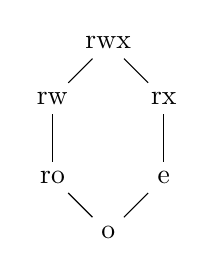
\begin{tikzpicture}[main node/.style={}]
  \node[main node] (1) {$\rwx$};
  \node[main node] (2) [below right of=1] {$\exec$};
  \node[main node] (3) [below of=2] {$\entry$};
  \node[main node] (4) [below left of=1] {$\readwrite$};
  \node[main node] (5) [below of=4] {$\readonly$};
  \node[main node] (6) [below right of=5] {$\noperm$};

  \path[every node/.style={font=\sffamily\small}]
    (1) edge (2)
    (2) edge (3)
    (3) edge (6)
    (1) edge (4)
    (4) edge (5)
    (5) edge (6);
\end{tikzpicture}
\caption{Permission hierarchy}
\label{fig:perm-hier}
\end{figure}
Notation:
$$\begin{array}{rcl}
i       &\in& \Instrs \\
r       &\in& \RegName\\
\mem    &::=& (\reg,\heap)\\
\pc     &\in& \Caps \\
\pcreg  &\in& \RegName \\
\Phi    &::=& \mem \in \Confs\\
\memheap&\in& \Heaps \\
\memreg &\in& \Regs \\
\addr   &\in& \Addrs\\
\perm   &\in& \Perms\\
(\perm,\start,\addrend,\addr) &\in& \Caps \\
n       &\in& \ints\\
\end{array}$$
Further definitions:
$$\begin{array}{rcl}
\lv    &::=& \refreg{r} \\
\hv    &::=& \refheap{r}\\
\rv    &::=& n \mid \lv \\
i      &::=& \fail \mid \halt \mid 
             \jmp{\lv} \mid \jnz{\lv}{\rv} \mid
             \isptr{\lv}{\rv} \mid \setptr{\lv}{\rv} \mid \\
       &   & \lea{\lv}{\rv} \mid\move{\lv}{\rv} \mid \load{\lv}{\hv} \mid \store{\hv}{\rv} \mid  \\
       &   & \restrict{\lv}{\rv}{\rv} \mid \subseg{\lv}{\rv}{\rv} \mid \plus{\lv}{\rv}{\rv}
\end{array}$$

\subsection*{Semantics}
Assume a $\decode$ function that decodes integer to instructions:
\begin{align*}
\decode &:\ints \rightarrow \Instrs
\end{align*}
Assume an $\encodePerm$ function that encodes a permission as an integer:
\begin{align*}
\encodePerm &: \Perms \rightarrow \ints
\end{align*}
\begin{align*}
  \Phi & \rightarrow \sem{\decode(\memreg(\pcreg))}(\Phi) & &                                   
                                                              \arraycolsep=0pt
                                                              \begin{array}{l}
                                                                \text{if $\memreg(\pcreg) = \stdcap$}\\
                                                                \quad\text{and $\start \leq \addr < \addrend$}\\
                                                                \quad\text{and $\perm \in \{ \exec,\rwx \}$ }
                                                              \end{array}\\
\Phi & \rightarrow \failed                                 & & \text{otherwise}
\end{align*}
It is assumed that address 0 is used for I/O, so whatever resides in location 0 after an execution can be seen as a result. As we will see in the semantics, it is assumed that the initial process starts with a readwrite capability for this location.
\begin{align*}
  \executeAllowed{\perm} &=
                           \begin{cases}
                             \true & \text{if } \perm \in \{ \rwx, \exec, \entry \} \\
                             \false & \text{otherwise}
                           \end{cases} \\
  \readAllowed{\perm} &=
                           \begin{cases}
                             \true & \text{if } \perm \in \{ \rwx, \exec, \readwrite, \readonly \} \\
                             \false & \text{otherwise}
                           \end{cases} \\
  \writeAllowed{\perm} &=
                           \begin{cases}
                             \true & \text{if } \perm \in \{ \rwx, \readwrite\} \\
                             \false & \text{otherwise}
                           \end{cases} \\
  \updatePcPerm{(\perm,\start,\addrend,\addr)} &=
                                     \begin{cases}
                                       (\exec,\start,\addrend,\addr) & \text{if $\perm = \entry$}\\
                                       (\perm,\start,\addrend,\addr) & \text{otherwise} 
                                     \end{cases} \\
  \nonZero{w} &=
                \begin{cases}
                  \true & \text{if $w\in \Caps$ or $w\in \ints$ and $w \neq 0$}\\
                  \false & \text{otherwise}
                \end{cases} \\
  \withinBounds{(\_,\start,\addrend,\addr)} &=
                                              \begin{cases}
                                                \true  & \text{if $\start \leq \addr \leq \addrend$} \\
                                                \false & \text{otherwise}
                                              \end{cases} \\
  \stdUpdatePc{\Phi} &=
                       \begin{cases}
                         \updateReg{\pcreg}{\var{newPc}} & 
                           \arraycolsep=0pt
                           \begin{array}{l}
                             \text{if $\memreg(\pcreg) = \stdcap$}\\
                             \quad\text{and $\var{newPc} = (\perm,\start,\addrend,\addr + 1)$}\\
                           \end{array} \\
                           \failed & \text{otherwise}
                       \end{cases} \\
\end{align*}
%TODO: \Phi.reg(rv) to some other notation. It should only look up reg, if it is a regname otherwise just the litteral.
\begin{align*}
  \sem{\fail}(\Phi)                        & = \failed \\
  \sem{\halt}(\Phi)                        & = (\halted,\Phi) \\
  \sem{\jmp{\lv}}(\Phi)                    & = \updateReg{\pcreg}{\updatePcPerm{\memreg(\lv)}} \\
  \sem{\jnz{\lv}{\rv}}(\Phi)               & = 
                                             \begin{cases}
                                               \updateReg{\pcreg}{\updatePcPerm{\memreg(\lv)}} &
                                               \arraycolsep=0pt
                                               \begin{array}{l}
                                                 \text{if $\nonZero{\memreg(\rv)}$} 
                                               \end{array}\\
                                               \stdUpdatePc{\Phi} & \text{if not $\nonZero{\memreg(\rv)}$}\\
                                               \failed & \text{otherwise }
                                             \end{cases} \\
 \sem{\load{\refreg{r_1}}{\refheap{r_2}}}  & = 
                                             \begin{cases}
                                               \stdUpdatePc{\updateReg{r_1}{\var{w}}} &
                                               \arraycolsep=0pt
                                               \begin{array}{l}
                                                 \text{if }\memreg(r_2) = (\perm,\start,\addrend,\addr) = \var{c} \\
                                                 \quad\text{and }\readAllowed{\perm} \text{ and } \withinBounds{\var{c}} \\
                                                 \quad\text{and }\var{w} = \memheap(\addr)
                                               \end{array}\\
                                               \failed & \text{otherwise }
                                             \end{cases}\\
 \sem{\store{\refheap{r_1}}{\refreg{r_2}}} & = 
                                             \begin{cases}
                                               \stdUpdatePc{\updateHeap{\addr}{\var{w}}} &
                                               \arraycolsep=0pt
                                               \begin{array}{l}
                                                 \text{if }\memreg(r_1) = (\perm,\start,\addrend,\addr) = \var{c} \\
                                                 \quad\text{and }\writeAllowed{\perm} \text{ and } \withinBounds{\var{c}} \\
                                                 \quad\text{and }\var{w} = \memreg(r_2)
                                               \end{array}\\
                                               \failed & \text{otherwise }
                                             \end{cases}\\
 \sem{\move{\refreg{r_1}}{\rv}}            & = \stdUpdatePc{\updateReg{r_1}{\memreg(\rv)}}
\\
  \sem{\lea{\refreg{r_1}}{\rv}}            & =
                                             \begin{cases}
                                               \stdUpdatePc{\updateReg{r_1}{\var{c}}} &
                                                 \arraycolsep=0pt
                                                 \begin{array}{l}
                                                   \text{if either $n = \rv$ or $\rv = \refheap{r_2}$ and $n = \memreg(r_2)$} \\
                                                   \quad\text{and in either case $n \in \ints $} \\
                                                   \quad\text{and $\memreg(r_1) = \stdcap$}\\
                                                   \quad\text{and $\var{c} = (\perm,\start,\addrend,\addr + n)$}
                                                 \end{array}\\
                                               \failed               & \text{otherwise}
                                             \end{cases} 
\\
 % In the M-Machine, lea checks whether the pointer stay within the allowed range in the pointer.
  \sem{\restrict{\refreg{r_1}}{\rv_1}{\rv_2}}           & =
                                             \begin{cases}
                                               \stdUpdatePc{\updateReg{r_1}{\var{c}}}  &
                                                 \arraycolsep=0pt
                                                 \begin{array}{l}
                                                   \text{if $\memreg(\rv_1) = c'$}\\
                                                   \quad\text{and $c' = \stdcap$}\\
                                                   \quad\text{and either $\rv_2 = n$ or $\memreg(\rv_2) = n$}\\
                                                   \quad\text{and in either case $n \in \ints$}\\
                                                   \quad\text{and $\var{newPerm} = \encodePerm(n)$}\\
                                                   \quad\text{and $\var{newPerm} \sqsubseteq \perm$}\\
                                                   \quad\text{and $c = (\var{newPerm},\start,\addrend,\addr)$}
                                                 \end{array}\\
                                               \failed                   & \text{otherwise}
                                             \end{cases} 
\end{align*}
\begin{align*}
  \sem{\plus{\refreg{r_1}}{\rv_1}{\rv_2}}               & =
                                                          \begin{cases}
                                                            \stdUpdatePc{\updateReg{r_1}{n_1+n_2}} &
                                                            \arraycolsep=0pt
                                                            \begin{array}{l}
                                                              \text{if for $i \in \{1,2\}$}\\
                                                              \quad\text{$n_i = \rv_i$ or $n_i = \memreg{\rv_i}$}\\
                                                              \quad\text{and in either case $n_i \in \ints$}
                                                            \end{array}\\
                                                            \failed & \text{otherwise}
                                                          \end{cases}\\
  \sem{\isptr{\lv}{\rv}} & = \undefined \\ 
  \sem{\setptr{\lv}{\rv}} & = \undefined \\ 
  \sem{\subseg{\lv}{\rv}{\rv}} & = \undefined 
\end{align*}

\section{Examples}
\label{sec:examples}
\subsection{Ticket Dispenser}
\label{sec:tick-disp}
\newcommand{\hsfoot}{\hs_\var{footprint}}
\newcommand{\hsframe}{\hs_\var{frame}}
\newcommand{\size}{\var{size}}
\newcommand{\rio}{r_{io}}
\newcommand{\adv}{\codelabel{adv}}
\newcommand{\advb}{\var{adv_{base}}}
\newcommand{\adve}{\var{adv_{end}}}
\newcommand{\initb}{\var{init}_{base}}
\newcommand{\inite}{\var{init}_{end}}
\newcommand{\mrlen}{5cm}
\newcommand{\retm}{\var{ret}_{\malloc}}
\newcommand{\reta}{\var{ret}_{\adv}}
\newcommand{\bracket}[1]{\multirow{#1}{*}{\ensuremath{
 \left . \vphantom{\begin{array}{l}
 \ifthenelse{\equal{#1}{1}}{3\\}{
    \ifthenelse{\equal{#1}{2}}{3\\3\\}{
    \ifthenelse{\equal{#1}{3}}{3\\3\\3\\}{
    \ifthenelse{\equal{#1}{4}}{3\\3\\3\\3\\}{
    \ifthenelse{\equal{#1}{5}}{3\\3\\3\\3\\3\\}{
    \ifthenelse{\equal{#1}{6}}{3\\3\\3\\3\\3\\3\\}{
      3\\3\\3\\3\\3\\3\\3\\ %7
  }}}}}}
  \end{array}} \right \}}}
}
\newcommand{\annotate}[2]{\multirow{#1}{\mrlen}{\scriptsize #2}}
Assume the instructions of some adversary resides in the memory starting at the memory location marked with $\advb$. Assume that the register $\rio$ initially contains a capability for the address in memory where I/O is written to (we assume this address is 0). We assume that entry capabilities for $\adv$ and $\malloc$ is ambiently available\dominique{what does this mean?}. The following is a test program for a ticket dispenser:
\[
  \begin{array}{r l l p{\mrlen}}
% Set io to -1
\initb:     & \store{\refheap{\rio}}{-1} & \bracket{1} & \annotate{1}{Initialize io to $-1$} \\
% Store io capability just after jump to adv
           & \move{\refreg{r_0}}{\refreg{\pcreg}} & \bracket{3} & \annotate{3}{Store the io capability on the stack} \\
           & \lea{\refreg{r_0}}{\iocap} & & \\
           & \store{\refheap{r_0}}{\refreg{\rio}} & & \\
% Overwrite io register
           & \move{\refreg{\rio}}{0} & \bracket{1} & \annotate{1}{Overwrite io register} \\
% Allocate memory for ticket dispenser program
           & \move{\refreg{r_1}}{\size} &  \bracket{4} & \annotate{4}{Allocate memory for the ticket dispenser program (including memory for counter and capability for counter)}\\
           & \move{\refreg{r_0}}{\refreg{\pcreg}} & & \\
           & \lea{\refreg{r_0}}{3} & & \\
           & \jmp{\malloc} & & \\
% Save ticket dispenser code
\retm:     & \store{\refheap{r_1}}{(\encode(i_1))} & \bracket{7} & \annotate{7}{Store the ticket dispenser program in the newly allocated memory} \\
           & \lea{\refreg{r_1}}{1} & & \\
           & \store{\refheap{r_1}}{(\encode(i_2))} & & \\
           & \lea{\refreg{r_1}}{1} & & \\
           & \vdots & & \\
           & \store{\refheap{r_1}}{(\encode(i_7))} & & \\
           & \lea{\refreg{r_1}}{1} & & \\
% Save capability for counter
           & \move{\refreg{r_0}}{\refreg{r_1}} & \bracket{4} & \annotate{4}{Store a capability for the counter address after the ticket dispenser program} \\
           & \lea{\refreg{r_0}}{1} & & \\
           & \store{\refheap{r_1}}{\refreg{r_0}} & & \\
           & \lea{\refreg{r_1}}{1} & & \\
% Save capability for counter two addresses after jump to adv.
           & \move{\refreg{r_2}}{\refreg{\pcreg}} & \bracket{3} & \annotate{3}{Store a capability for the counter in this code} \\
           & \lea{\refreg{r_2}}{\counter} & & \\
           & \store{\refheap{r_2}}{r_0} & & \\
           & \move{\refreg{r_2}}{0} & \bracket{1} & \annotate{1}{Overwrite capability for counter} \\
% Save counter
           & \store{\refheap{r_1}}{0} & \bracket{1} & \annotate{1}{Initialize counter to 0} \\
% Change pointer to point to start of ticket dispenser code
           & \lea{\refreg{r_1}}{-8} & \bracket{1} & \annotate{1}{Capability points to start of td code \footnote{This is also the argument for the adversary}} \\
% Set up entry pointer to ticketDispenser for adv.
           & \restrict{\refreg{r_1}}{\refreg{r_1}}{(\encodePerm{(\entry)})} &\bracket{1} & \annotate{1}{Restrict cap. to td} \\
% Set up return pointer
           & \move{\refreg{r_0}}{\refreg{\pcreg}} & \bracket{3} & \annotate{3}{Setup a return pointer for the adversary} \\
           & \lea{\refreg{r_0}}{5} & & \\
           & \restrict{\refreg{r_0}}{\refreg{r_0}}{(\encodePerm{(\entry)})} & & \\
% jump to adv
           & \jmp{\adv} & \bracket{1} & \annotate{1}{Jump to the adversary} \\
           & 0 & \bracket{1} & \annotate{1}{Address reserved for io cap.} \\
           & 0 & \bracket{1} & \annotate{1}{Address reserved for counter cap.} \\
% retrieve io capability
\reta:     & \move{\refreg{r_0}}{\refreg{\pcreg}} & \bracket{3} & \annotate{3}{Retrieve the io capabiltiy} \\
           & \lea{r_0}{-2} & & \\
           & \load{\refreg{\rio}}{\refheap{r_0}} & & \\
% retieve counter capability
           & \lea{r_0}{1} & \bracket{2} & \annotate{2}{Retrieve the counter capability} \\
           & \load{\refreg{r_1}}{\refheap{r_0}} & & \\
% load the value of the counter
           & \load{\refreg{r_0}}{\refheap{r_1}} & \bracket{2} & \annotate{2}{Read the counter and write it to io address} \\
% store the value of the counter to io
           & \store{\refheap{\rio}}{\refreg{r_0}} & & \\
\inite :   & \halt
  \end{array}
\]
Here $\size$ is 9. The variables $\counter$ and $\iocap$ are respectively the offsets to the addresses reserved for the counter and io capabilities. $i_1 \dots i_7$ refers to the instructions in the following ticket dispenser:
\[
  \begin{array}{r l}
    i_1 :& \move{\refreg{r_2}}{\refreg{\pcreg}} \\
    i_2 :& \load{\refreg{r_2}}{\size - 2} \\
    i_3 :& \load{\refreg{r_1}}{\refheap{r_2}}\\
    i_4 :& \plus{\refreg{r_3}}{\refreg{r_1}}{2} \\
    i_5 :& \store{\refheap{r_2}}{\refreg{r_3}} \\
    i_6 :& \move{\refreg{r_2}}{0} \\
    i_7 :& \jmp{\refreg{r_0}}
  \end{array}
\]
The heap layout for the above program can be seen in Figure~\ref{tab:tick-disp-heap}.
\begin{figure}[ht]
  \centering
  \begin{tabular}{ | c | l | }
    \hline
    Addr. & Content \\ \hline
    0   &  $i_1$ \\ \hline
    1   &  $i_2$ \\ \hline
    2   &  $i_3$ \\ \hline
    3   &  $i_4$ \\ \hline
    4   &  $i_5$ \\ \hline
    5   &  $i_6$ \\ \hline
    5   &  $i_7$ \\ \hline
    7   & Cap. for addr. 8 \\ \hline
    8   & The counter \\ \hline  
  \end{tabular}
  \caption{The heap layout for the ticket dispenser.}
  \label{tab:tick-disp-heap}
\end{figure}

In the JS paper, the ticket dispenser program dereferences the counter and returns the value. It does not seem like a similar thing would work here as the adversary can do even more. In particular, the adversary can execute a $\halt$ instruction that will cause the machine to halt (successfully). The adversary could also choose never to return to the return address that we set up for him.
\begin{lemma}[Ticket dispenser test]\dominique{I would prefer more precise, symbolic statements of assumptions and less prose.}
\label{lem:tckt-disp}
 Given a configuration $\Phi$, if
 \begin{description}
 \item[$\boldsymbol \memheap$] contains the ticket dispenser test program starting at the address labelled $\initb$, 
 \item[$\boldsymbol \memheap$] contains the adversary code starting at label $\advb$. The adversary is assumed to have no capabilities on the heap, but it has access to the ambient $\malloc$ capability! \lau{maybe mention that malloc is also on the heap}
 \item[$\boldsymbol \memheap$] contains the malloc code, and the malloc code satisfy $\iota_{\malloc}$, i.e., $\forall n \ldotp \heapSat[{\heap\restrictfun{\{\malloc_{\var{base}}, \dots ,\malloc_{\var{end}}\}}}]{n}{W_{\malloc}}$.
 \item[All the above programs are disjoint.]
 \item[$\boldsymbol{\adv}$ and $\boldsymbol{ \codelabel{malloc}}$] capabilities are ambiently available at all times.
 \item[$\boldsymbol{ \memreg(\pcreg)}$] is $(\rwx,\initb,\inite,\initb)$.
 \item[$\boldsymbol{ \memreg(\rio)}$] is $(\readwrite,0,0,0)$.
 \item[the remaining registers] all contains 0,
 \end{description}
 and $\Phi \rightarrow^* (\halted,\Phi')$, then the I/O address (that is $\memheap[\Phi'](0)$) contains either $-1$ or a number that is $\geq 0$ and even.
\end{lemma}
In the initial configuration the $\pcreg$ register is assumed to have an execute and write permission for the area of the heap where the program resides.

The ticket dispenser test program uses $\malloc$. To be able to reason about programs that use $\malloc$, we assume that it follows the following specification. If you provide it with one argument, namely the size of the allocation you wish and a return capability, then at some point $\pcreg$ will contain an executable capability based on this return capability and the return register will contain a $\rwx$ capability for the freshly allocated memory. 
\begin{specification}[Malloc v.2]
  \begin{align*}
    &\forall \Phi \in \Mems \ldotp \forall \hsfoot, \hsframe \in \HeapSegments\ldotp\\
    &\quad \forall n, i, \size \in \nats\ldotp\forall b,e,a,m_b,m_e\in \Addrs\ldotp\forall p \in \Perms \ldotp\\
    &\qquad W_{\malloc} = [i \mapsto \iota_{\malloc}] \land \\
    &\qquad \dom(\hsfoot) = [m_b,m_e] \land \\
    &\qquad \memheap = \hsfoot \uplus \hsframe \land\\
    &\qquad \heapSat[\hsfoot]{n}{W_{\malloc}} \land \\
    &\qquad \memreg(r_1) = \size \land \\
    &\qquad \size \geq 0 \land \\
    &\qquad \memreg(r_0) = (p,b,e,a) \land \\
    &\qquad \memreg(\pcreg) = (\entry,m_b,m_e,m_b) \\
    &\qquad\Rightarrow \\
    &\qquad \quad\exists \Phi' \in \Mems \ldotp \exists \hsfoot' \in \HeapSegments\ldotp\\
    &\qquad \qquad \exists j,k \in \nats \ldotp \exists b',e'\in \Addrs \ldotp \\
    &\qquad \qquad \quad \Phi \step[j]\Phi' \land \\
    &\qquad \qquad \quad \memheap[\Phi']=\hsfoot' \uplus \hsframe \land\\
    &\qquad \qquad \quad W' = [i \mapsto \iota_{\malloc}, k \mapsto \iota^0_{b',e'}] \land \\
    &\qquad \qquad \quad \heapSat[\hsfoot']{n-j}{W'} \land \\
    &\qquad \qquad \quad \memreg[\Phi'](\pcreg) = (\updatePcPerm{p},b,e,a) \land \\
    &\qquad \qquad \quad \size = e'-b'
    &\qquad \qquad \quad \memreg[\Phi'](r_1) = (\rwx,b',e',b') \land \\
    &\qquad \qquad \quad \forall r \in \RegName \setminus \{\pcreg,r_1\} \ldotp \memreg[\Phi'](r) = 0
\end{align*}
\end{specification}
\lau{I am not satisfied with the pc in the premise. The exact capability necessary very much depent on the implementation (this is mostly a note to myself.)}
\dominique{I agree with the remark about the pc.  Perhaps leave the form of the
  pc unspecified as it is not important for malloc users?}
\dominique{Resulting frame should be equal to original.}
\dominique{Allocated pointer should have the right size.}
\dominique{Other registers unmodified could be an alternative. (Caller-save/Callee-save etc.)}

\begin{specification}[Malloc]\dominique{can you state this more systematically, with less prose, more explicit assumptions and conclusion?}
Take $W_{\malloc}$ the world with exactly one island, namely the unspecified island $\iota_{\malloc}$ that governs the internal state of $\malloc$.  If we invoke $\malloc$ in a memory $h = \hsframe \uplus \hsfoot$
%\lau{Is $\hsframe$ supposed to be the rest of memory, so $h$ is something we can execute in? Is $\malloc$ allowed to allocate more memory, i.e., how does $\hsfoot$ relate to $\hsfoot'$?} A: The frame contains anything that has been allocated and the footprint contains the rest. That is the footprint contains mallocs internal state as well as the free memory.
% Notice: the current worlds do not support malloc allocating memory as the invariants cannot evolve.
that is the disjoint sum of a frame part and a footprint part and the latter satisfies this world up to steps $n$, i.e., $\heapSat[\hsfoot]{n}{W_{\malloc}}$. Then $\malloc$ will successfully terminate and return a result in a heap $h' = \hsframe \uplus \hsfoot'$ that is the disjoint sum of the same unmodified frame part and a potentially new footprint part, such that there is a future world $W'$ of $W_{\malloc}$ consisting of exactly two islands, where the first is an instance of $\iota_{\malloc}$ and the second is the region $\iota_{\var{base},\var{end}}^0$
%\lau{doesn't this invariant allow the newly allocated memory to contain capabilities?} A: It does not capture this. One possiblity is to make new standard all zero invariant.
 for an appropriately-sized interval $\var{base},\var{end}$ and the new footprint part satisfies this new world $\heapSat[\hsfoot']{n}{W'}$. 
%\lau{at what step should this hold? Just some step $n'<n$?} A: try with n, if that does not work, then say something like: there exists j such that malloc terminates in j steps and use n-j.
%\lau{It should probably be more precise what it means to ``invoke'' $\malloc$ and for $\malloc$ to ``return'' something.} A: yes. If we won't abstract notion of this, the standard way to formulate it would be with Hoare triples.
%\lau{How do we express that $\malloc$ can be ``trusted'' in the sense that it won't save any capabilities like one to the newly allocated memory or the return capability.} A:  it allows for read capabilities! To capture this, we need either non-interference or some kind of trace semantics!

To \emph{invoke} $\malloc$ means that the capability in $\pcreg$ points to a $\jmp{\malloc}$ instruction (and that this address is within its capabilities). Further in the register $r_0$ there has to be a return capability, i.e., a capability of the form $(\perm,\var{returnStart},\var{returnEnd},\var{returnAddr})$ where $\perm$ is either, $\rwx$, $\exec$, or $\entry$. Lastly, the register $r_1$ has to contain the argument for $\malloc$ which is the desired length of the piece of memory to be allocated.

To \emph{return} from $\malloc$ means that the register $\pcreg$ contains the capability $(\perm',\var{returnStart},\var{returnEnd},\var{returnAddr})$ where $\perm'$ is $\rwx$ if $\perm$ was $\rwx$ and $\exec$ otherwise. Further, register $r_1$ contains $(\rwx,\var{base},\var{end},\var{base})$ which is a capability for the allocated memory. 
\end{specification}

 \begin{proof}[Proof (Lemma~\ref{lem:tckt-disp})]
Let configuration $\Phi$ be given where the heap is shaped as follows:
\begin{itemize}
\item $\memheap$ contains the ticket dispenser test program (tdtp) starting at address $\initb$.
\item $\memheap$ contains the adversary code starting at address $\advb$ and ending at address $\adve$. The adversary code contains no capabilities.
\item $\memheap$ contains the malloc code.
\item (and so on) %TODO write the remaining assumptions
\end{itemize}
and the register file contains:
\begin{enumerate}
\item $\memreg(\rio) = (\readwrite,0,0,0)$ 
\item $\memreg(\pcreg) = (\rwx,\initb, \inite, \initb)$
\item $\memreg(r) = 0$ for the remaining registers $r$ in the register file.
\end{enumerate}

If we start running in $\Phi$ until $\jmp{\malloc}$ has just been executed, then the configuration is the same as $\Phi$ except:
\begin{itemize}
\item $\memheap(0)$ contains $-1$
\item the io capability is saved to the designated address in the tdtp
\item $r_1$ contains the size of the ticket dispenser program (9)
\item $r_0$ contains the return capability $(\rwx,\initb,\inite, \retm)$
\end{itemize}
Call this new heap $\Phi'$

To be able to say something about the jump to $\malloc$, we use its specification. Take $\hsfoot$ to be the part of the heap $\malloc$ resides in and everything that has not been allocated according to the assumptions. Take $\hsframe$ to be everything else. We have $\heapSat[\hsfoot]{n}{W_\var{\malloc}}$ as the world only has one region, namely the one that governs $\malloc$.\dominique{explicit assumption about this needed?} According to the specification of $\malloc$, we get $\Phi' \step^* \Phi''$ where
\begin{itemize}
\item $\memheap[\Phi'] = \hsframe \uplus \hsfoot'$
\item $\memreg[\Phi'](r_1) = (\rwx,\var{base},\var{end},\var{base})$ for some addresses $\var{base}$ and $\var{end}$
\item $\memreg[\Phi'](\pcreg) = (\rwx,\initb,\inite,\retm)$
\end{itemize}
Further for $W'$ with exactly two regions $\iota_\malloc$ and $\iota_{\var{base},\var{end}}^0$ we have that the new footprint satisfies this world, i.e., $\heapSat[\hsfoot']{n}{W'}$.

If we continue running from $\Phi'$ until just after the point we have executed $\jmp{\adv}$, then  $\pcreg$ points to an execute capability for the adversary, and  we reach a configuration $\Phi''$ which is the same as $\Phi$ except:
\begin{itemize}
\item $\memheap[\Phi''](0)$ contains $-1$
\item capabilities for \emph{the counter} and io are saved to the designated addresses in the tdtp
\item the ticket dispenser code resides on the heap starting at the address $\var{base}$ (the code is as seen in Figure~\ref{tab:tick-disp-heap})
\item $\memreg[\Phi''](\pcreg) = (\exec,\advb,\adve,\advb)$
\item $\memreg[\Phi''](r_0) = (\entry,\initb,\inite,\reta)$
\item $\memreg[\Phi''](r_1) = (\entry,\var{base},\var{end},\var{base})$
\item all other registers contain 0
\end{itemize}
We now want to use the FTLR. To do so, we need to define a world that represents our current heap. We pick the following world:
\begin{itemize}
\item $\iota_{\var{io}}$ the region governs the heap segment that only has address $0$. The value of address $0$ should be $-1$ or $\geq 0$ and even.  % The region that governs that output address
\item $\iota_{\var{td}}$ this region governs heap segments with the domain $[\var{base},\var{end}]$ for the addresses $[\var{base},\var{end} - 1]$ they are the same as in $\Phi''$. $\hs(\var{base})$ is positive and even.
\item $\iota_{\var{tdtp}}$ this region governs the ticket dispenser test programs. The domain of a heap segment in this region is that of the ticket dispenser test program and the contents of the heap segment should be the same as it is in $\Phi''$.
\item $\iota_{\advb,\adve}$
\item $\iota_{\malloc}$
\end{itemize}
To use the FTLR, we have to argue that the read condition is satisfied for the region, the adversary is in. This is easily shown, as we have chosen the region for the adversary to be the standard one, so with $\advb$ and $\adve$ as witnesses, we need to show $\iota_{\advb,\adve} \subseteq \iota_{\advb,\adve}$.

So we can conclude that $\npair{(\exec,\advb,\adve,\advb}) \in \stder(W'')$ where $W''$ is the world with the following regions:
Assuming we can show the following three things:
\begin{enumerate}
\item $\memreg[\Phi''] \in \stdrr(W'')$
\item $\npair{c = (\exec,\initb,\inite,\reta)}] \in \stdkr(W'')$
\item $\heapSat[{\memheap[\Phi'']}|]{n}{W''}$ where the we have limited the heap to the segments governed by the regions in $W''$.
\end{enumerate}
then it follows from the fact that the adversary program is in the expression predicate that
\[
\npair{\Phi^{(3)} = (\updateReg[\Phi'']{r_0}{c}[\plainproj{reg}.r_1 \mapsto (\exec,\advb,\adve,\advb)].\plainproj{reg},\memheap[\Phi''])} \in \observations(W'').
\]
From this and the fact that we know the execution terminates, we know that $\Phi^{(3)} \step^k (\halted,h)$ for some heap $h$ and $k \leq n$. From this we can conclude that the heap segment that only consists of address 0 is accepted by region $\iota_{\var{io}}$ which means that either $h(0)$ is $-1$ or positive and even which is exactly what the lemma says.

It remains to show that 1-3 holds. For 1, all registers but $r_0$ and $r_1$ are easy as they contain $0$ which is always in the value predicate. For $r_0$ and $r_1$, we do need to do some reasoning. Both capabilities have one things in common, namely that the underlying programs do not use the arguments.

$\memreg[\Phi''](r_0)$ contains the capability $(\entry,\initb,\inite,\reta)$ and we need to show that it is in $\stdvr(W'')$. Let $n' < n$ and $W^{(3)} \future W''$ be given and show $\npair[n']{(\exec,\initb,\inite,\reta)} \in \stder(W^{(3)})$. Let $\reg \in \stdrr(W^{(3)})$, $\npair[n']{c} \in \stdkr(W^{(3)})$, $\heapSat[\heap]{n'}{W^{(3)}}$ and $\heap_f$ be given. We do not really care about the register file and the continuation as the ticket dispenser test program does not use them. As $\heap$ satisfies $W^{(3)}$, parts of the heap must satisfy the invariants $\iota_{\var{tdtp}}$ and $\iota_{\var{td}}$ which means the ticket dispenser program and the ticket dispenser test program is unaltered. It also means that the counter in the ticket dispenser is $\geq 0$ and even. We need to show $\npair[n']{(\reg[r_0 \mapsto c][r_1 \mapsto ](\exec,\initb,\inite,\reta), \heap \uplus \heap_f)} \in \observations(W^{(3)})$. If $n'$ is sufficiently small, then we run out of steps before the program halts in which case the configuration is trivially in the $\observations$ predicate. If the execution halts successfully, then the ticket dispenser test program will have moved the value of the counter in the ticket dispenser to address 0, the designated I/O address. As this is a numerical value, it will trivially be in the value predicate. Further, the island that governs address 0 is $\iota_{\var{io}}$, so we have to argue that the value is $\geq 0$ and even. The value came from the ticket dispenser which is governed by the region $\iota_{\var{td}}$ so it is indeed $\geq 0$ and even.

In register $r_1$ we have the capability $(\entry,\var{base},\var{end},\var{base})$ and we need to show $\npair[n]{(\exec,\var{base},\var{end},\var{base})} \in \stder(W'')$. To this end, we go through the same motion as for $r_0$:  Let $n' < n$, $W^{(3)} \future W''$, $\reg \in \stdrr(W^{(3)})$, $\npair[n']{c} \in \stdkr(W^{(3)})$, $\heapSat[\heap]{n'}{W^{(3)}}$ and $\heap_f$ be given. Show 
\[
\npair[n']{(\reg[r_0 \mapsto c][r_1 \mapsto ](\exec,\var{base},\var{end},\var{base}), \heap \uplus \heap_f)} \in \observations(W^{(3)}).
\]
Again the heap satisfaction makes sure that the ticket dispenser program is as we expect, so we can execute it. If we run out of steps before we reach $\jmp{\refreg{r_0}}$, then it is in the observation predicate. Otherwise, we reach a new configuration $\Phi^{(3)}$ where the registers are the same as in $\reg$ except for $r_0$, $r_1$, $r_2$, and $\pcreg$ which will be $c$, the previous counter value, $0$, and $\updatePcPerm(c)$ respectively. $0$ is trivially in the value predicate and $c$ is in the value predicate as it is in the continuation predicate, so $\reg$ is in the register-file predicate. If we split the heap part of $\Phi^{(3)}$ into the same two parts as we had in the initial assumption, then we need to argue that the non-frame part still satisfies the world. The only change made to the heap was updating the counter. The heap segments that did not change still satisfy their regions. We have to argue that the heap segment $[\var{base},\var{end}]$ still satisfies the region $\iota_{\var{td}}$. The ticket dispenser code remains unchanged and the counter is $\geq 0$ and even as it was computed by adding two to a value which was $\geq 0$ and even, so the ticket dispenser heap segment satisfies $\iota_{\var{td}}$. Now we have all the necessary conditions satisfied to be able to use the fact that $c$ is in the continuation predicate to conclude 

\lau{did I mess up the steps here?}
\[
\npair[n']{(\reg\update{r_0}{c}\update{\pcreg}{\updatePcPerm{c}}, \heap' \uplus \heap_f)} \in \observations
\]
(where $\heap'$ is the new heap). From this we get that continuing from the configuration we end up with no more steps, failing, or in a halting state that satisfies the world.

%condition 2

\dominique{this duplicates the argument about $(\entry,\initb,\inite,\initb+\var{ret}) \in \stdvr(W'')$. Find a way to share this?}
For condition 2, we need to show 
\[
\npair{c = (\entry, \initb, \inite,\reta)}] \in \stdkr(W'').
\]
To this end, let $W^{(3)} \future W''$, $\reg \in \stdrr(W^{(3)})$, $\heapSat[\heap]{n'}{W^{(3)}}$ and $\heap_f$ be given. We then need to argue 
\[
\npair{(\reg\update{\pcreg}{\updatePcPerm{c}},\heap \uplus \heap_f)} \in \observations(W^{(3)}).
\]
As part of the heap satisfies a future world of $W''$, we know that the ticket dispenser test program remains unaltered. If we run it (and do not run out of steps), then it loads the couner, stores it to address $0$, and halts. From the heap satisfaction, we get that the counter is positive and even, so the value we store to address 0 is positive and even. The value is trivially in the value relation as it is an integer. Further the region that governs address 0 is $\iota_{\var{io}}$ which requires the value there to be positive and even which it is. So in this case the configuration is in the observation predicate. If we run out of steps, then it is also in the observation relation.

%condition 3
Finally, we need to show $\heapSat[{\memheap[\Phi'']}|]{n}{W''}$. The domains of the heap segments are assumed to be disjoint, and we have limited the heap to only be the parts considered in the regions, so the first condition of heap satisfaction is okay. Let us take the regions one at a time and briefly argue that the corresponding heap segment satisfies the region:
\begin{itemize}
\item $\iota_{\var{io}}$ governs address 0, which i initial $-1$. This region requires it to be $-1$ or $\geq 0$ and even, so it is initially satisfied.
\item $\iota_{\var{tdtp}}$, this region was constructed so the part of the heap it governs remains unaltered.
\item $\iota_{\var{td}}$, apart from the address with the counter, this region is also constructed so this heap segment does not change. With respect to the counter, it requires it to be $\geq 0$ and even. The counter starts as 0, so also this cell satisfies the region.
\item $\iota_{\advb,\adve}$ the adversary code is assumed to be instructions only which are trivially satisfied by the standard island.
\item $\iota_{\malloc}$, from the specification of $\malloc$ we got that the resulting heap after the allocation satisfied a world with $\iota_{\malloc}$. We use the same region and we have not changed that part of the heap, so it still satifies this region.
\end{itemize}

We have now shown the three conditions and thus proven Lemma~\ref{lem:tckt-disp}.
\end{proof}

\section{Logical Relation}
\label{sec:logical-relation}
\subsection{Worlds}
\[
  \StorePred = \Worlds \monnefun \UPred{\Addrs \parfun \Words}
\]
\[
\Worlds \cong \frac{1}{2} (\RegionName \parfun \StorePred)
\]

A standard heap invariant that insures all values in the region are in the value  relation:
\[
  \iota_{\var{start},\var{end}} \; : \; \StorePred
\]
\begin{align*}
  \iota_{\var{start},\var{end}}(W) \defeq  \{ \npair{\heapseg} \mid & \dom(\heapseg) = [\var{start},\var{end}] \land \\
                                                               & \quad \forall \addr \in \dom(\heapseg) \ldotp \npair{\heapseg(\addr)} \in \stdvr(W) \}
\end{align*}
Another standard heap invariant that ensures all the words in the region are 0.
\[
  \iota_{\var{start},\var{end}}^0 \; : \; \StorePred
\]
\begin{align*}
  \iota_{\var{start},\var{end}}^0(W) \defeq \{ \npair{\heapseg} \mid & \dom(\heapseg) = [\var{start},\var{end}] \land \\
                                                                & \qquad \forall \addr \in \dom(\heapseg) \ldotp \heapseg(\addr) = 0  \}
\end{align*}


\begin{align*}
  \readCond{n,W,\start,\addrend} =        & \;\exists r \in \RegionName \ldotp \\
                                          & \;\quad \exists [\start',\addrend'] \supseteq [\start,\addrend] \ldotp W(r) \nsubeq[n-1] \iota_{\start',\addrend'} \\ & \\
  \writeCond{n,W,\start,\addrend} =       & \; \exists r \in \RegionName \ldotp \\
                                          & \;\quad \exists [\start',\addrend'] \supseteq [\start,\addrend] \ldotp W(r) \nequal[n-1] \iota_{\start',\addrend'} \\ & \\
  \execCond{n,W,\start,\addrend,\perm} =  & \; \forall n' < n \ldotp \forall W' \future W \ldotp \\
                                          & \; \quad \forall \addr \in [\start,\addrend] \ldotp \\
                                          & \; \qquad \npair[n']{(\perm,\start,\addrend,\addr)} \in \stder(W') \\ & \\
  \entryCond{n,W,\start,\addrend,\addr} = & \; \forall n' < n \ldotp \forall W' \future W \ldotp \\
                                          & \; \quad \npair[n']{(\exec,\start,\addrend,\addr)} \in \stder(W') \land \\
\end{align*}

\begin{lemma}[Write condition implies read condition]
\[
\forall n, W, \start, \addrend \ldotp \writeCond{n,W,\start,\addrend} \Rightarrow \readCond{n,W,\start,\addrend}
\]
\end{lemma}
\[
\stdvr \; : \;  \Worlds \monfun \UPred{\Words}
\]
\begin{align*}
  \stdvr(W) \defeq & \{ \npair{i} \mid i \in \ints \} 
\union \\
                   & \{ \npair{\stdcap[\noperm] }  \} 
\union \\
                   & \{ \npair{\stdcap[\readonly] } \mid \readCond{n,W,\start,\addrend} \} \union \\
                   & \{ \npair{\stdcap[\readwrite] } \mid \writeCond{n,W,\start,\addrend} \} \union \\
                   & \{ \npair{\stdcap[\exec]} \mid \\
                   & \quad\readCond{n,W,\start,\addrend} \land \\
                   & \quad \execCond{n,W,\start,\addrend,\exec} \}
\union \\
% For the entry case a capability is acceptable, if we can change it to an execute permission and put it as the pc and we otherwise have valid words in the registers, then the register file should be valid.
                   & \{ \npair{\stdcap[\entry]} \mid \entryCond{n,W,\start,\addrend} \} \union \\
                   & \{ \npair{\stdcap[\rwx]} \mid \\
                   & \quad \writeCond{n,W,\start,\addrend} \land \\
                   & \quad \execCond{n,W,\start,\addrend,\exec} \land \\
                   & \quad \execCond{n,W,\start,\addrend,\rwx} \}
\end{align*}

Consider what the ``good observations'' should be? Before we do that - what should the end result of a computation be?
\begin{align*}
  \observations \quad : & \quad  \Worlds \monfun \UPred{\Regs \times \HeapSegments} \\
  \observations (W) \defeq & \{ \npair{(\reg,\hs)} \mid \\
                           & \quad (\forall \heap_f, \heap', i \leq n \ldotp (\reg,\hs \uplus \heap_f) \step[i] (\halted,\heap')  \\
                           & \qquad \Rightarrow \exists \hs' \ldotp \heap' = \hs' \uplus \heap_f \land \heapSat[\hs']{n-i}{W}
\end{align*}
Removed the condition $\npair[n-i]{\heap'(0)} \in \stdvr(W)$.\\

The ``good observations'' are as follows
\begin{itemize}
\item The execution does not stop in $n$ steps. 
\item The execution stops with a $\failed$.
\item The execution halts in at most $n$ steps with a heap where the island that governs address 0 is satisfied by some heap segment.
\end{itemize}
Address 0 is the designated I/O address.

Register-file relation:
\begin{align*}
  \stdrr \quad : & \quad \Worlds \monfun \UPred{\Regs} \\
  \stdrr(W) \defeq & \{ \npair{\reg} \mid \\
                    & \quad \forall r \in \RegName \setminus \{\pcreg\} \ldotp \\
                    & \qquad  \npair{\reg(r)} \in \stdvr(W) \}
\end{align*}

``Continuation'' relation:
\begin{align*}
  \stdkr \quad : & \quad  \Worlds \monfun \UPred{\Words} \\%TODO: Check if this is still monotone
  \stdkr(W) \defeq & \{ \npair{c} \mid c \in \stdvr(W) \land \\
                   & \quad \forall W' \future W, n' < n\ldotp %on the whiteboard, we had public future world.
                     \forall \heapSat[\hs]{n'}{W'} \ldotp \forall \reg \in \stdrr(W') \\
                   & \qquad \npair[n']{(reg\update{\pcreg}{\updatePcPerm{\var{c}}},hs)} \in \observations(W') \}
\end{align*}
We require the continuation to be in the value relation, because it will have to be in the registers when it is invoked, so to argue that the register file is in the register-file relation, we need to know that the continuation is in the value relation.

Normally, it would just be required for the return value to be in the value relation, so the continuation is invoked with this value. Here everything that is in the register file is available when the continuation is invoked, so we do not special case on $r_1$ (which is the register that in the calling convention we use should contain the return value). 

``Expression'' relation:
\begin{align*}
  \stder \quad : & \quad \Worlds \monfun \UPred{\Words} \\%TODO: Check whether this needs to be monotone
  \stder(W) \defeq & \{ \npair{\pc} \mid \\
                   & \quad \forall \npair{\reg} \in \stdrr(W) \ldotp \\
                   & \qquad \forall \npair{c} \in \stdkr(W) \ldotp \\
                   & \qquad \quad  \forall \heapSat[\hs]{n}{W} \ldotp \\
                   & \qquad \qquad \npair{(\reg\update{r_0}{c}\update{\pcreg}{\pc},\hs)} \in \observations(W) \}
\end{align*}

\begin{definition}[Heap satisfaction/erasure]
\begin{align*}
  \heapSat{n}{W} & & \text{iff} & &
                                      \arraycolsep=0pt
                                      \begin{array}{l}
                                      \exists r: \dom(W) \rightarrow \HeapSegments \ldotp \\
                                      \qquad\heap = \biguplus_{\iota\in \dom(W)} r(\iota)\\
                                      \quad\text{and}\\
                                      \qquad\forall \iota \in \dom(W) \ldotp \npair{r(\iota)} \in W(\iota)(W)
                                      \end{array}\\
\end{align*}

\end{definition}
\begin{lemma}[Fundamental theorem of logical relations (FTLR)] \forcenewline
  For any $n \in \nats$, $W \in \Worlds$, $p\in \Perms$, and addresses $\var{base}$, $\var{end}$, and $a$, if $\perm = \rwx$ and $\writeCond{n,W,\var{base},\var{end}}$ or $\perm = \exec$ and $\readCond{n,W,\var{base},\var{end}}$, then $\npair{(\perm, \var{base}, \var{end}, a)} \in \stder(W)$.
\end{lemma} %TODO: Change the condition here to be writeCondition (and readCondition)
\lau{With the current definition of the expression relation, an entry pointer will never be in the expression relation, but I guess we do not want that restriction. Say the adv capability in the ticket dispenser lemma, we want that to be an entry capability.}
\lau{In the ticket dispenser lemma, we need to make some assumptions about the adversary to be able to use the FTLR. What should these assumptions be? So far I have the assumption that it is all code (no capabilities), but I do not see how I conclude the write condition from this.}
\dominique{Something I find interesting here, is that the FTLR can be interpreted to say that x permissions have no real security value: if you have an arbitrary r or rw capability that is valid, then the FTLR says that it remains valid if we change it to rx or rwx (respectively).}

\begin{lemma}[Heap satisfaction downwards closure]
\[
  \forall n,n',\heap, W \ldotp \heapSat{n}{W} \land n' < n \Rightarrow \heapSat{n'}{W}
\]
\end{lemma}

\begin{lemma}[Read condition downwards closure]
\[
\forall n,n',W,\start, \addrend \ldotp \readCond{n,W,\start,\addrend} \land n' \leq n \Rightarrow \readCond{n',W,\start,\addrend}
\]
\end{lemma}
\begin{lemma}[Write condition downwards closure]
\[
\forall n,n',W,\start, \addrend \ldotp \writeCond{n,W,\start,\addrend} \land n' \leq n \Rightarrow \writeCond{n',W,\start,\addrend}
\]
\end{lemma}


\section{Related reading}
\label{sec:related-reading}

This is a list of related work that might be interesting to read in the context
of this project.

\subsection{Capability machines}
\label{sec:rw-cap-machines}

\subsubsection{M-Machine}
More than 20 years ago, \cite{Carter:1994:HSF:195473.195579} have described the
use of capabilities in the M-Machine. They do seem to have a reference for the
instruction set after all~\citep{Dally1997Memo59}; it seems like the server was
just temporarily down when we were looking for this the first time...

\subsubsection{CHERI}

The CHERI processor is a much more recent capability machine, described
by~\cite{Woodruff:2014:CCM:2665671.2665740,Watson2015Cheri}.

Another result of this project is also CheriBSD: an adaptation of FreeBSD to the
CHERI
processor.\footnote{\url{http://www.cl.cam.ac.uk/research/security/ctsrd/cheri/cheribsd.html}}
It is not separately described in a published paper, but mentioned in the papers
cited above and in some tech reports (see url). This work includes a
pure-capability ABI that could provide some interesting examples.

The CHERI team also has a webpage with all of their CHERI-related publications
(including TRs and
such)\footnote{\url{http://www.cl.cam.ac.uk/research/security/ctsrd/cheri/}}.

\subsection{Logical Relations}
\label{sec:rw-log-rel}

Some papers on logical relations that are relevant for this work are the
following:

\cite{Hur:2011:KLR:1926385.1926402} describe a logical relation between ML and
a (standard) assembly language for expressing compiler correctness.  Relevant
because they target an assembly language, and they use biorthogonality.

\cite{Dreyer:2010:IHS:1863543.1863566} describe a logical relation for a ML-like
language and use public/private transitions to reason about well-bracketed
control flow. Relevant because we are considering to cover an example of
enforcing well-bracketed control flow in a capability machine.

\cite{Devriese:2016ObjCap} describe a logical relation for a JavaScript-like
language with object capabilities.  Relevant because it treats object
capabilities, albeit in a JavaScript-like lambda calculus.

\bibliographystyle{plainnat}
\bibliography{refs}

\end{document}
